\documentclass[10pt]{scrreprt}
\usepackage[utf8]{inputenc}
\usepackage{amsfonts}
\usepackage{amsmath}
\usepackage{amssymb}
\usepackage{commath}
\usepackage[ngerman]{babel}
\usepackage{enumitem}
\usepackage{booktabs}
\usepackage{longtable}
\usepackage{relsize}
\usepackage{pgfplots}
\usepackage{csvsimple}
\usepackage{pgfplotstable}
\usepackage{siunitx}
\usepackage{fancyhdr}
\usepackage{color}
\usepackage{float}
\usepackage{listings}
\usepackage{graphicx}
\usepackage{subcaption}
\usepackage[europeanresistors]{circuitikz}

\definecolor{mygreen}{RGB}{28,172,0} % color values Red, Green, Blue
\definecolor{mylilas}{RGB}{170,55,241}


\lstset{language=Matlab,%
%basicstyle=\color{red},
breaklines=true,%
morekeywords={matlab2tikz},
keywordstyle=\color{blue},%
morekeywords=[2]{1}, keywordstyle=[2]{\color{black}},
identifierstyle=\color{black},%
stringstyle=\color{mylilas},
commentstyle=\color{mygreen},%
showstringspaces=false,%without this there will be a symbol in the places where there is a space
%numbers=left,%
%numberstyle={\tiny \color{black}},% size of the numbers
%numbersep=9pt, % this defines how far the numbers are from the text
emph=[1]{for,end,break},emphstyle=[1]\color{red}, %some words to emphasise
%emph=[2]{word1,word2}, emphstyle=[2]{style},
}

\setlength\parindent{0pt}

\setcounter{chapter}{5}
\setcounter{secnumdepth}{3}
\setcounter{section}{0}

\pagestyle{fancy}
\fancyhf{}
\lhead{GPET Versuch 10}
\rhead{Tim Luchterhand, Paul Nykiel}
\cfoot{\thepage}

\author{Tim Luchterhand, Paul Nykiel \protect\\ tim.luchterhand@uni-ulm.de, paul.nykiel@uni-ulm.de}
\title{GPET Versuch 10 --- Zuse und Lilienfeld – ganz diskret}
\subtitle{Gruppe: Dienstag14}

\begin{document}
    \maketitle

    \section{Relais-Inverter mit Widerstand}
    Im ersten Teil des Versuchs soll das 12V-Relais untersucht werden. Achten Sie beim An-
    schließen der Eingangsspannung an die Spule des Relais immer auf die richtige Polarität.
    Diese ist zwar prinzipiell bei einem Relais irrelevant, allerdings wurde hier eine Diode par-
    allel zur Spule verlötet um induktionsbedingte Spannungsspitzen bei den Schaltvorgängen
    kurzzuschließen. Um nun nicht die Eingangsspannung selbst kurzzuschließen, muss unbe-
    dingt auf entsprechende Polarität geachtet werden.

    \subsection{Stromverbrauch des Relais}
    Das Relais wird zunächst mit konstanter Versorgungsspannung betrieben, dabei soll der
    Stromverbrauch gemessen werden.
    \begin{figure}[H]
        
\includegraphics[width=\textwidth]{abb11.png}
        \caption{Aufbau: Relais mit konstanter Versorgung}
        \label{fig:abb11}
    \end{figure}

    \begin{enumerate}
        \item Arbeiten Sie mit der konstanten Gleichspannung $U_{DD} = +10\si{\volt}$.
            Begrenzen Sie den Strom auf $100\si{m\ampere}$.
        \item Bauen Sie die Schaltung aus Abbildung~\ref{fig:abb11} bestehend aus dem Relais und dem
            Multimeter zur Strommessung auf.
        \item Wie viel Strom fließt durch die Spule des Relais?
    \end{enumerate}

    \subsection{Dynamik des Relais}
    Um die Tauglichkeit des Relais als Schalter für die Digitaltechnik zu untersuchen, wird
    im Folgenden ein Inverter nach Abbildung~\ref{fig:abb12} aufgebaut. Das dynamische Verhalten des
    Bauelements soll unter Verwendung eines Testsignals untersucht werden.

    \begin{figure}[H]
        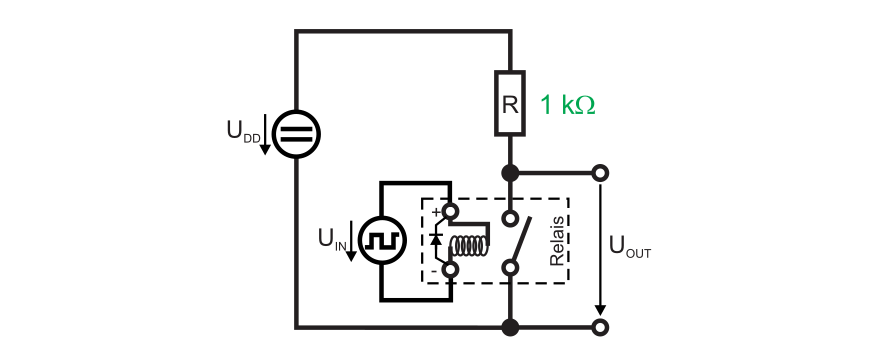
\includegraphics[width=\textwidth]{abb12.png}
        \caption{Aufbau: Relais mit Pull-Up-Widerstand}
        \label{fig:abb12}
    \end{figure}

    \begin{enumerate}
        \item Verwenden Sie eine Gleichspannung von $+10\si{\volt}$ als Versorgung $U_{DD}$.
            Begrenzen Sie den Strom auf $100\si{m\ampere}$.
        \item Zur Generierung des Testsignals $U_{IN}$ soll der externe Funktionsgenerator verwendet
            werden. Erzeugen Sie ein Rechtecksignal mit den Potentialgrenzen $0\si{\volt}$ und $+10\si{\volt}$
            bei einer Frequenz von $10\si{\hertz}$. Messen Sie mit dem Oszilloskop auf Kanal 1 zunächst
            das Testsignal und prüfen Sie dessen Richtigkeit. Schließen Sie das Relais zu diesem
            Zeitpunkt noch nicht an und stellen Sie vor Allem sicher, dass das untere Limit von
            $0\si{\volt}$ nicht unterschritten wird.
        \item Bauen Sie die Inverterschaltung aus Abbildung~\ref{fig:abb12} auf. Verwenden Sie den 1 kOhm
            Widerstand als Pull-Up.
        \item Messen Sie mit dem Oszilloskop auf Kanal 2 den Schaltungsausgang $U_{OUT}$.
            Untersuchen Sie die Reaktionszeit des Relais (nicht die Anstiegs- \& Abfallzeit!). Fügen
            Sie entsprechende Screenshots vom Oszilloskop in Ihr Protokoll mit ein.
            \begin{itemize}
                \item \textbf{
                        Wie lange dauert es, bis ausgangsseitig stabil $+10\si{\volt}$ anliegen, wenn
                        der Schaltungseingang auf niedriges Potential gefallen ist?
                    }
                \item \textbf{
                        Wie lange dauert es, bis ausgangsseitig stabil $0\si{\volt}$ anliegen, wenn
                        der Schaltungseingang auf hohes Potential gestiegen ist?
                    }
                \item \textbf{
                        Ermitteln Sie, basierend auf diesen Messungen, die zu erwartende
                        maximale Frequenz mit der das Relais gerade noch arbeiten kann.
                    }
                \item \textbf{
                        Verifizieren Sie den berechneten Wert in der Praxis. Bei welcher
                        Frequenz kann das Relais gerade noch arbeiten?
                    }
            \end{itemize}
    \end{enumerate}

    \section{nMOS-Inverter mit Widerstand}
    Es wird nun an Stelle des elektromechanischen Bauelements der rein elektrisch
    arbeitende Transistor verwendet. Dabei soll die theoretisch besprochene Problematik der
    Widerstandsdimensionierung anhand eines Inverters praktisch verdeutlicht werden. Der Inverter
    wird dabei auf Stromverbrauch, Ausgangsspanne und Schaltgeschwindigkeit untersucht.

    \subsection{Stromverbrauch und Ausgangsspanne des nMOS-Inverters}
    \begin{figure}[H]
        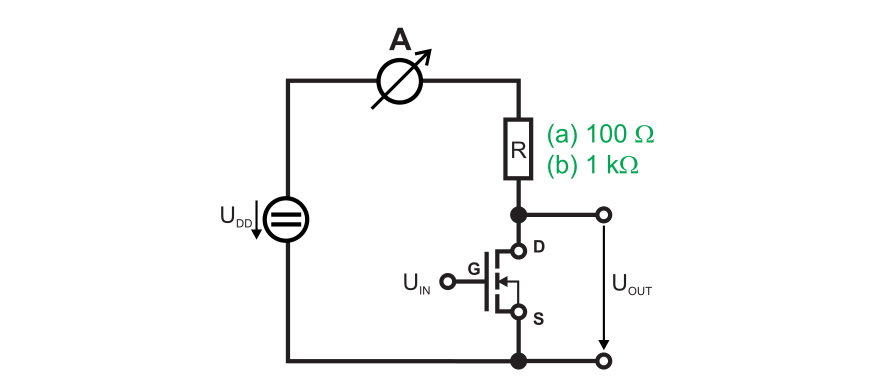
\includegraphics[width=\textwidth]{abb13.png}
        \caption{Aufbau: nMOS-Inverter mit Widerstand, konstante Eingangsspannung}
        \label{fig:abb13}
    \end{figure}

    \begin{enumerate}
        \item Verwenden Sie jetzt eine Gleichspannung von $+5\si{\volt}$ als Versorgungsspannung $U_{DD}$.
            Stellen Sie die Spannung mit Hilfe eines Multimeters möglichst genau ein. Entfernen
            Sie danach das Multimeter wieder. Begrenzen Sie den Strom auf $100\si{m\ampere}$.
        \item Bauen Sie die Schaltung aus Abbildung~\ref{fig:abb13} mit einem n-Kanal MOSFET auf.
            Verwenden Sie zunächst 100 Ohm als Pull-Up.
        \item Legen Sie den Schaltungseingang $U_{IN}$ auf das feste Potential \textit{GND}.
            \textbf{Messen Sie  die Ausgangsspannung $U_{OUT}$ in diesem Zustand.Messen Sie außerdem
            den Strom, der dabei verbraucht wird.}
        \item Verbinden Sie $U_{IN}$ nun mit der Versorgungsspannung. \textbf{Messen Sie erneut die
            Ausgangsspannung $U_{OUT}$ und den Stromverbrauch des Inverters.}
        \item Tauschen Sie den Widerstand $R$ aus. Verwenden Sie jetzt den 1 kOhm - Widerstand
            und wiederholen Sie die Messungen aus den vorigen beiden Schritten.
            Beachten Sie, welche Werte sich ändern.
            %TODO Tabellen
    \end{enumerate}


    \subsection{Dynamik des nMOS-Inverters}
    \begin{figure}[H]
        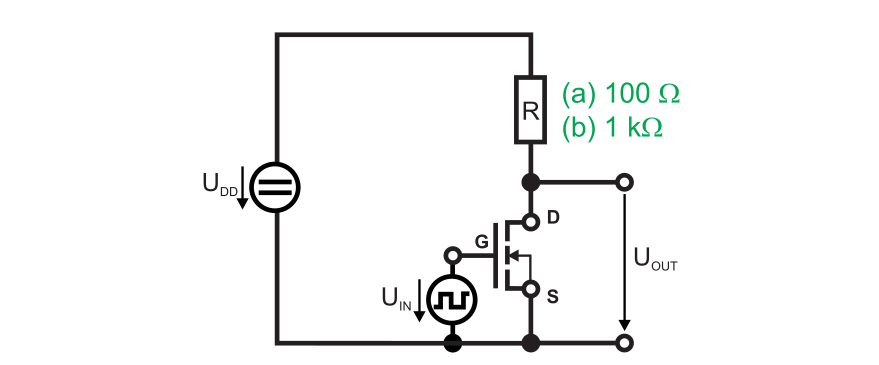
\includegraphics[width=\textwidth]{abb14.png}
        \caption{Aufbau: nMOS-Inverter mit Widerstand, Dynamikuntersuchung}
        \label{fig:abb14}
    \end{figure}
    \begin{enumerate}
        \item Arbeiten Sie weiterhin mit der Gleichspannung von $+5\si{\volt}$ als Versorgungsspannung
            $U_{DD}$. Begrenzen Sie den Strom auf $100\si{m\ampere}$.
        \item Zur Generierung des Testsignals $U_{IN}$ soll ab jetzt der interne Frequenzgenerator
            des Oszilloskops verwendet werden. Erzeugen Sie ein Rechtecksignal mit den
            Potentialgrenzen $0\si{\volt}$ und $+5\si{\volt}$ bei einer Frequenz von $1\si{M\hertz}$. Messen Sie mit dem
            Oszilloskop auf Kanal 1 zunächst das Testsignal und prüfen Sie dessen Richtigkeit.
            Schließen Sie das Eingangssignal an wie in Abbildung~\ref{fig:abb14} dargestellt, verwenden Sie
            hierfür ein BNC-Kabel.
        \item Untersuchen Sie die Schaltung aus Abbildung~\ref{fig:abb14}. Verwenden Sie zunächst 100 Ohm
            als Pull-Up. Entfernen Sie unbedingt das Amperemeter vom vorigen Versuch aus
            der Schaltung, dieses würde die nachfolgenden Untersuchungen verfälschen.
            \begin{figure}[H]
                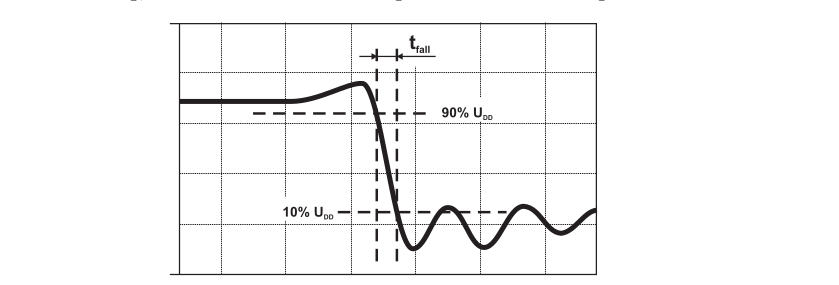
\includegraphics[width=\textwidth]{abb15.png}
                \caption{Messung der Schaltzeiten}
                \label{fig:abb15}
            \end{figure}
        \item Messen Sie mit dem Oszilloskop auf Kanal 2 über ein weiteres BNC-Kabel den
            Schaltungsausgang $U_{OUT}$. Untersuchen Sie die Anstiegs- \& Abfallzeit der Schaltung.
            Führen Sie die Messungen durch wie in Abbildung~\ref{fig:abb15} gezeigt. Messen Sie die Zeit
            für das Fallen oder Steigen des Ausgangssignals zwischen 10\% und 90\% der Versorgungsspannung.
            Verwenden Sie die Cursor-Funktion des Oszilloskops manuell, da
            die automatische Messung der Anstiegs- \& Abfallzeit durch das hohe Schwingungsverhalten
            der Schaltung meist überfordert ist.
            \begin{itemize}
                \item \textbf{
                        Wie lange dauert es, ausgehend von 10\% $U_{DD}$, bis ausgangsseitig
                        erstmals 90\% $U_{DD}$ anliegen (Anstiegszeit, $t_{rise}$)?
                    }
                \item \textbf{
                        Wie lange dauert es, ausgehend von 90\% $U_{DD}$, bis ausgangsseitig
                        erstmals 10\% $U_{DD}$ anliegt (Abfallzeit, $t_{fall}$)?
                    }
                \item \textbf{
                        Bestimmen Sie die theoretische Maximalfrequenz mit der die Schaltung,
                        basierend auf den Messungen, gerade noch funktionieren kann.
                    }
            \end{itemize}
        \item Tauschen Sie den Widerstand $R$ aus. Verwenden Sie nun 1 kOhm. \textbf{Messen Sie
            erneut die Schaltzeiten.}
            %TODO Tabelle
        \item \textbf{
                Nennen Sie Vor- \& Nachteil(e) eines großen Pull-Up-Widerstands.
                }
    \end{enumerate}

    \section{CMOS Grundschaltungen}
    \subsection{CMOS-Inverter}
    Um die CMOS-Logik mit den vorher untersuchten Technologien vergleichen zu können,
    wird auch in diesem Versuch zunächst ein Inverter aufgebaut. Dabei wird der Pull-Up-
    Widerstand ganz einfach durch einen p-Kanal MOSFET ersetzt.

    \subsection{Stromverbrauch und Ausgangsspanne des CMOS-Inverters}
    \begin{figure}[H]
        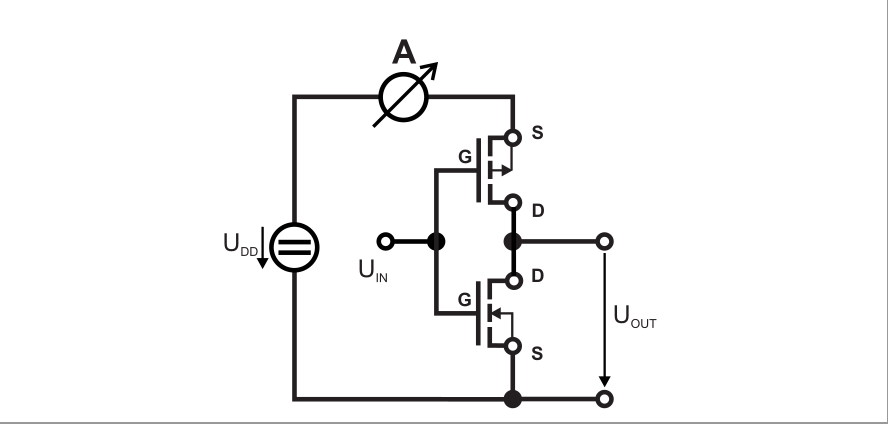
\includegraphics[width=\textwidth]{abb16.png}
        \caption{Aufbau: CMOS-Inverter, konstante Eingangsspannung}
        \label{fig:abb16}
    \end{figure}
    \begin{itemize}
        \item Verwenden Sie $+5\si{\volt}$ als Versorgung $U_{DD}$ mit Strombegrenzung auf $100\si{m\ampere}$.
        \item Bauen Sie die Schaltung aus Abbildung~\ref{fig:abb16} mit einem n-Kanal MOSFET und einem
            p-Kanal MOSFET auf.
        \item Legen Sie den Schaltungseingang $U_{IN}$ auf festes Potential \textit{GND}. \textbf{Messen Sie die
            Ausgangsspannung $U_{OUT}$. Messen Sie den Strom, den der Inverter verbraucht.}
        \item Verbinden Sie $U_{IN}$ mit der Versorgungsspannung. \textbf{Messen Sie erneut
            Ausgangsspannung $U_{OUT}$ und Stromverbrauch des Inverters.}
            %TODO Tabelle
        \item \textbf{Vergleichen Sie die Ergebnisse mit denen des nMOS-Inverters.}
    \end{itemize}

    \subsection{Dynamik des CMOS-Inverters}
    \begin{figure}[H]
        
\includegraphics[width=\textwidth]{abb17.png}
        \caption{Aufbau: CMOS-Inverter, Dynamikuntersuchung}
        \label{fig:abb17}
    \end{figure}
    \begin{enumerate}
        \item Verwenden Sie weiter $+5\si{\volt}$ für $U_{DD}$. Begrenzen Sie den Strom auf $100\si{m\ampere}$.
        \item Das Testsignal $U_{IN}$ soll erzeugt werden, wie im Versuch mit dem nMOS-Inverter.
            Generieren Sie ein Rechtecksignal mit Potentialgrenzen $0\si{\volt}$ und $+5\si{\volt}$ bei einer
            Frequenz von $1\si{M\hertz}$.
        \item Untersuchen Sie die Schaltung aus Abbildung~\ref{fig:abb17} (entfernen Sie das Amperemeter).
        \item Messen Sie mit dem Oszilloskop auf Kanal 2 den Schaltungsausgang $U_{OUT}$. Untersuchen
            Sie abermals die Dynamik. Führen Sie die Messung durch wie beim nMOS-Inverter.
            \begin{itemize}
                \item \textbf{
                        Messen Sie die Anstiegszeit $t_{rise}$.
                    }
                \item \textbf{
                        Messen Sie die Abfallzeit $t_{fall}$.
                    }
                \item \textbf{
                        Bestimmen Sie die theoretische Maximalfrequenz mit der die
                        Schaltung, basierend auf den Messungen, gerade noch funktionieren kann.
                    }
            \end{itemize}
        \item \textbf{
            Welche Bauweise für einen Inverter würden Sie vorziehen? Vergleichen
            Sie die untersuchten Varianten und begründen Sie Ihre Wahl.
        }
    \end{enumerate}

    \subsection{CMOS-NOR}
    \begin{itemize}
        \item Verwenden Sie eine Gleichspannung von $+5\si{\volt}$ als Versorgungsspannung $U_{DD}$.
            Begrenzen Sie den Strom auf $100\si{m\ampere}$.
        \item Bauen Sie das CMOS-NOR entsprechend Ihrer Vorbereitung auf.
        \item Verifizieren Sie die Wahrheitstabelle, indem Sie die Eingänge $U_A$ und $U_B$
            entsprechend mit den Potentialen \textit{GND} und $U_{DD}$ belegen.

            \vspace{0.1cm}

            \textbf{
                Messen Sie den Schaltungsausgang mit dem Multimeter und vergleichen
                Sie mit der Tabelle aus ihrer Vorbereitung.
            }
    \end{itemize}

\end{document}
